\section{Robustness and Generalization within a Domain}

An interesting observation from Figure~\ref*{fig:stylometry_extensions:followingTrail:results:rq1_zeroshot} is that the performance of the LUAR model on the Reddit data is worse on the dataset collected in 2019 compared to the dataset collected in 2018.
In light of this observation, in this section, we are concerned with evaluating the impact of temporal data drift, latent author demographic attributes, and their interaction on authorship attribution.
We find that both the time elapsed between writing samples and latent demographic attributes can have a significant impact on performance, which we attribute to temporal data shifts.
Further, we find that these shifts are more significant for certain groups, notably younger authors whose style evolves over time.
This is problematic since these groups may suffer from higher error rates and suffer potential negative outcomes, such as false attributions in forensic applications.
Our experiments suggest this degradation in performance is due to fundamental data shifts, rather than model estimation error, which motivates us to propose a recalibration-based mechanism to improve the robustness of authorship attribution models.

\subsection{Motivation}

The objective of contrastive training is to learn a mapping from an input space---writing samples in our case---to a lower dimensional vector space wherein distance between feature vectors implies a measure of semantic similarity. 
For example, supervised contrastive learning, which is employed by several models evaluated in this work, uses labels associated with each example to ``pull'' representations sharing the same semantic label closer together, while ``pushing'' representations for examples with different semantic labels further apart~\cite{khosla2020supervised}. 

For authorship representation learning, we use author labels as supervision, and we interpret the vector similarity as a measure of the likelihood that two writing samples have the same author. 
The contrastive training objective can be thought of as attempting to enforce certain \emph{invariances} on the learned representations.
In the case of authorship, we desire representations that are invariant to text attributes that exhibit large variance for a single author, such as the particular topics being written about, while capturing stable author features such as writing style, which are more constant over time~\cite{andrews2019learning}.
However, although recent work has successfully improved performance of author representations in downstream tasks, such as social media account linking, for example by training on datasets comprising millions of anonymous authors~\cite{khan2021deep}, their limitations remain poorly understood. 
Section~\ref{chp:stylometry_extensions:followingTrail} describes some limitations of these models in their domain generalization capabilities.

As another step to better understand these limitations, in this section we focus on two central questions. 
First, do author representations capture representations that allow author identification to generalize across time?
Through careful experiment design, we find that the degradation in author identification performance may originate from temporally evolving styles rather than model estimation error.
Second, do author representations encode systematic biases associated with author demographics? 
We answer this question in the affirmative, finding that authorship attribution performance degrades significantly across demographic groups, including age and gender. 

\subsection{Datasets}
We start from the Pushshift Reddit dataset~\cite{baumgartner2020pushshift} generating the different splits. 
%by filtering for users who had at least  comments for user modeling over time. 
%Additionally, we filtered out users having more than 10,000 posts in an attempt to exclude bots. 
We restricted the time period of the data from January 2015 to November 2019.
In each setting, we follow a query/target temporal setup similar to previous work on retrieval-based authorship verification~\cite{andrews2019learning,khan2021deep}.
That is, we first selected a set of users and then include all the posts written by each selected user across two non-overlapping time periods.
The author identification task in such a setting takes a user's posts from the query time period as input and outputs a list of users ranked by their likelihood of matching the query user using their posts from the target time period.
A positive match requires having a top/high rank for the posts by the same user during the target time period.
We constructed multiple such datasets to help quantify the robustness of authorship attribution models.
Specifically, we created two types of datasets: TemporalReddit and DemographicReddit.

\subsubsection{TemporalReddit} 
In each dataset, we sampled users having between $p_{\rm{min}}$ and $p_{\rm{max}}$ posts in both the query and the target period. 
Specifically, we selected query/target temporal pairs with a fixed time difference between them.
Suppose the queries span time period $(Q_{\rm{start}}, Q_{\rm{end}}) = (q_1, q_2)$ and the targets span $(T_{\rm{start}}, T_{\rm{end}}) = (t_1, t_2)$.
We ensured that $\Delta_\tau = q_2 - t_2$ was similar across all datasets. 
However, we varied $q_1$ to obtain multiple, non-overlapping datasets.
We chose queries from January 2015 to January 2019 (5 query sets, each one month long) and targets from December 2015 to December 2018 and October 2019 with $p_{\rm{min}} = 16, p_{\rm{max}} = 2000$ with a set of 50k users sampled for each query-target pair.
In the following texts, we refer to these datasets as \DSfixeddelta{}.
A degradation in performance of author identification models over \DSfixeddelta{} would suggest that model estimation is not stable to temporal data shifts, and that the model would need to be retrained to maintain performance over time.
For the second dataset, we selected a single, fixed query split and multiple target splits. 
The query period chosen was Jan 2015, and the target periods chosen were Dec 2015--2018, Oct 2019. 
We sampled a set of 50k users having $p_{\rm{min}} = 16, p_{\rm{max}} = 2000$ in the query as well as in each target split.
We refer to this dataset as \DSvarydelta{}. 
A degradation in performance in \DSvarydelta{} would indicate that temporal changes of author style lead to a degradation in performance of author identification models.

\subsubsection{DemographicReddit}

\begin{table}[h]
    \centering
    \begin{tabular}{lrr}
    \toprule
    group & fraction & count \\
    \midrule
    adult & 0.52 & 1575 \\
    teenager & 0.39 & 1195 \\
    senior & 0.02 & 66 \\
    middle-aged & 0.05 & 164 \\
    %adult & 0.525000 & 1575 \\
    %teenager & 0.398333 & 1195 \\
    %senior & 0.022000 & 66 \\
    %middle-aged & 0.054667 & 164 \\
    \bottomrule
    \end{tabular}
    \caption{Distribution of demographics for age groups in \DSagefixed{}.}
    \label{tab:demographics:age_dist}
\end{table}

\begin{table}[]
    \centering
    \begin{tabular}{lrr}
    \toprule
    gender & fraction & count \\
    \midrule
    f & 0.51 & 614 \\
    m & 0.49 & 586 \\
   % f & 0.511667 & 614 \\
   % m & 0.488333 & 586 \\
    \bottomrule
    \end{tabular}
    \caption{Distribution of demographics for gender in \DSgenderfixed{}.}
    \label{tab:demographics:gender_dist}
\end{table}

We used the RedDust dataset~\cite{tigunova2020reddust} to collect self-identified demographic attributes associated with Reddit users. 
Specifically, we investigated two latent demographic attributes (age and gender) and their correlation with author identifiability.
We followed the authors' original definition for categorizing users into age groups (13-23: Teenager, 24-45: Adult, 45-65: Middle-Aged, 65+: Senior).
To create each of these datasets, we first subset the data to include only those users who lie in the intersection of our subset of the Pushshift dataset with RedDust-Age and RedDust-Gender. 
Following this, we selected a sequence of consecutive monthly splits from these intersecting users having $p_{min} = 8$ for at least five consecutive months. 
We restricted the users to be present across all the splits to ensure that the demographics do not change over splits.
Furthermore, to control for temporal variation, we only considered query/target pairs from consecutive months, i.e., $T_{start} - Q_{start} = 1~\rm{month}$.
We select a sequence of months that ensure that we can maximize the number of users with known demographics from RedDust.
The selected splits under this constraint corresponded to the months of January to May 2019.
We sampled 3k users' posts from this period with known age, giving us \DSagefixed{}, and 1.2k users' posts with known gender, \DSgenderfixed{}, derived from RedDust-Age and RedDust-Gender, respectively.
Note that the age in the data was adjusted to reflect the age of the user in January 2019 for all splits.

\subsubsection{TDReddit}
In addition to constructing query/target pairs with a fixed $T_{start} - Q_{start} = 1~\rm{month}$, we can additionally consider all possible pairs of query/target from the splits collected for creating the DemographicReddit datasets.
These pairs correspond to $\Perm{5}{2} = 20$ query/target pairs.
The two corresponding demographic datasets are labeled \DSagevary{} and \DSgendervary{} for age and gender, respectively.
%\pmcomment{TODO}

\subsection{Experiments}\

\subsubsection{Baselines}

We describe the models used and the rationale for the choice of these models in the following text.
The first three models correspond to count-based baselines that do not use neural networks for representation learning.
The final three models correspond to neural network-based models that use different representation learning model for each window, and these representations are merged in a LUAR like setup (Figure~\ref{fig:stylometry_extensions:followingTrail:LUAR}).
Similar baselines have been used in other work on author identification~\cite{wang2023can,soto2024fewshot}.

\noindent \textbf{Count-Subreddit (CS):}
The CS model uses a count based representation of each author, where each entry of the of the author representation vector represents the number of times the author posted on the corresponding subreddit.
In particular, we use the CountVectorizer from \citet{scikit-learn}. %with 10000 features, lower casing, and a minimum document frequency of 0.8.
Subreddit usually represent a topic of interest, so this vector could be seen as a simple proxy for the topics the author is interested in.

\noindent \textbf{TFIDF-Subreddit (TFS)}:
The TFS model uses TFIDFVectorizer from scikit-learn with the subreddits that an author posts in as the `term'.
This is another compact representation of the topics of interest for an author.

\noindent \textbf{TFIDF-Text (TFT)}:
The TFT model uses all the text posted by an author coverts it into a TF-IDF vector (also using the TFIDFVectorizer) over the text posted by each author as input.
This vector captures both topics, as well as some aspects of style such as word usage frequencies.

The hyperparameters for the aforementioned models were chosen using a grid search over the hyperparameter space with a separate split of the query/target data.

\noindent \textbf{SBERT} The popular sentence transformer model SBERT~\cite{reimers2019sentencebert} is used to generate the representation for each window of text for an author.
The representations from this model may capture the semantics and syntax associated with the text posted by the author.


\noindent \textbf{STEL} The STEL model from \citet{wegmann2021capture}, which is a modular framework to represent linguistic style while controlling for content, is used to generate the representation for each window of text for an author.
This model focuses on features that capture writing style only.

\noindent \textbf{LUAR} This is the LUAR model from~\cite{riverastao2021learning}. 
This model is trained to represent time invariant features of an author's writing style.

\begin{comment}
\pmComment{Consider whether to include the probing classifier expts - not particularly informative}
\subsubsection{Probing Classifier}
In order to test for bias present in the representations themselves, we train a probing classifier on each model's embeddings. A probing classifier is often used as a means of interpreting a deep neural network's ability to encode a particular property (see \citet{belinkov2022} for a thorough overview). If the classifier performs well, the property is presumably encoded in the embeddings and thus is assumed to play a role in the neural network's performance on the main task. Probing classifiers have some limitations, such as uncertainty over how to interpret the classifier's performance, %and the classifier's use of a property not necessarily correlating to the neural network's use of that property 
but for our exploratory purposes, we include the experiment as an indication of potential explanations for the models' performance.

We train logistic regression classifiers on the LUAR, SBERT, and STEL representations and test the classifiers' performance on 1) distinguishing gender and 2) distinguishing age. If a classifier performs well at distinguishing either demographic feature, it would seem that that feature is encoded in the embeddings to some degree. 
\end{comment}

\subsection{Evaluation and Discussion}

\subsubsection{TemporalReddit}

\begin{table*}[th]
    \centering
%\begin{tabular}{lrrrrrr}
%#\toprule
%#method & OS & TFS & TFT & SBERT & STEL & LUAR \\
%#Q/T &  &  &  &  &  &  \\
%#\midrule
%#15-1/15-12 & 0.236660 & 0.260280 & 0.191880 & 0.232300 & 0.135340 & \textbf{0.778740} \\
%#16-1/16-12 & 0.265440 & 0.283820 & 0.212460 & 0.250740 & 0.148480 & \textbf{0.795860} \\
%#17-1/17-12 & 0.278040 & 0.297200 & 0.223520 & 0.262440 & 0.137220 & \textbf{0.732580} \\
%#18-1/18-12 & 0.283220 & 0.302520 & 0.231700 & 0.280600 & 0.171020 & \textbf{0.769940} \\
%#19-1/19-10 & 0.315960 & 0.343180 & 0.234520 & 0.289820 & 0.143080 & \textbf{0.759620} \\
%#\bottomrule
%\end{tabular}
\begin{tabular}{lrrrrrr}
    \toprule
method & CS & TFS & TFT & SBERT & STEL & LUAR \\
Q/T &  &  &  &  &  &  \\
\midrule
15-1/15-12 & 0.237 & 0.260 & 0.192 & 0.232 & 0.135 & 0.779 \\
16-1/16-12 & 0.265 & 0.284 & 0.212 & 0.251 & 0.148 & 0.796 \\
17-1/17-12 & 0.278 & 0.297 & 0.224 & 0.262 & 0.137 & 0.733 \\
18-1/18-12 & 0.283 & 0.303 & 0.232 & 0.281 & 0.171 & 0.770 \\
19-1/19-12 & 0.316 & 0.343 & 0.235 & 0.290 & 0.143 & 0.760 \\
\bottomrule
\end{tabular}
    %\caption{Recall@8 results across different models on \DSfixeddelta{}. Only LUAR is controlled for training dataset time. Best performance is bolded.   }
    \caption{Recall@8 results across different models on \DSfixeddelta{}. The leftmost column represents the Query/Target period.}
    \label{tab:temporal_fixed}
\end{table*}

Table~\ref{tab:temporal_fixed} shows the evaluation results of recall@8 for \DSfixeddelta{}. LUAR significantly outperforms all other models across all fixed time periods.
As expected, the TFIDF and count based models, which do not require explicit `training' for data in a specific time period, have relatively stable author identification performance over time.
The results from the SBERT/STEL models, which are not trained without controlling the time periods for the training dataset, also show a similar trend.
As LUAR is trained on data from 2015-2016, if the author representations were overfit to identify authors in this time period, we would expect a significant drop in performance for the later time periods.
The last column on the right of Table~\ref{tab:temporal_fixed} shows that this is not the case, and LUAR's performance is relatively stable across time.
Thus, for a consistent query-target time difference, LUAR is able to maintain a high level of performance across time periods, indicating that model retraining is not necessary to maintain performance over time.
%\pmComment{Need better presentation option for this}

% TODO: At least make this a faceted plot 
\begin{figure}[ht]
    \centering
    \begin{subfigure}{0.48\linewidth}
    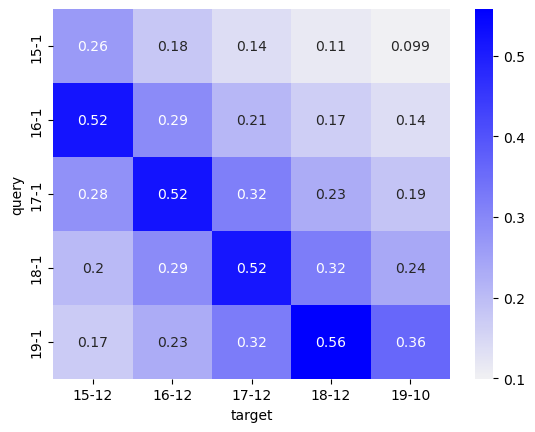
\includegraphics[width=\linewidth]{stylometryExtensions/figures/heat/os.png}
    \caption{CS}
    \label{fig:tempral_vary:os}
    \end{subfigure}
    \begin{subfigure}{0.48\linewidth}
    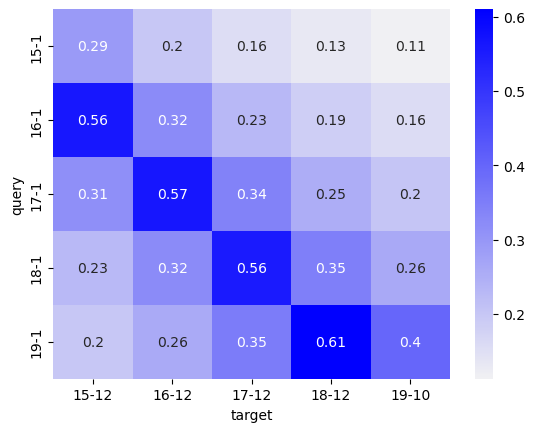
\includegraphics[width=\linewidth]{stylometryExtensions/figures/heat/tfs.png}
    \caption{TFS}
    \label{fig:tempral_vary:tfs}
    \end{subfigure}
    
    \begin{subfigure}{0.48\linewidth}
    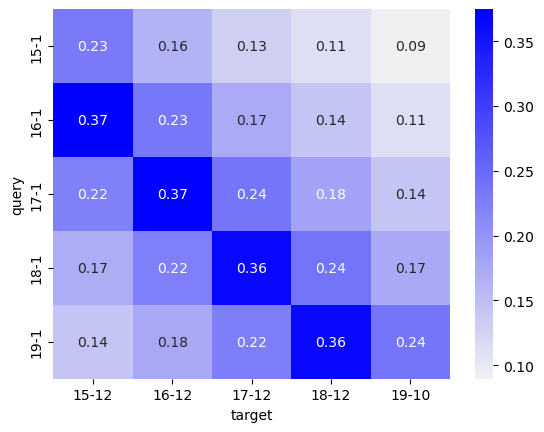
\includegraphics[width=\linewidth]{stylometryExtensions/figures/heat/tft.png}
    \caption{TFT}
    \label{fig:tempral_vary:tft}
    \end{subfigure}
    \begin{subfigure}{0.48\linewidth}
    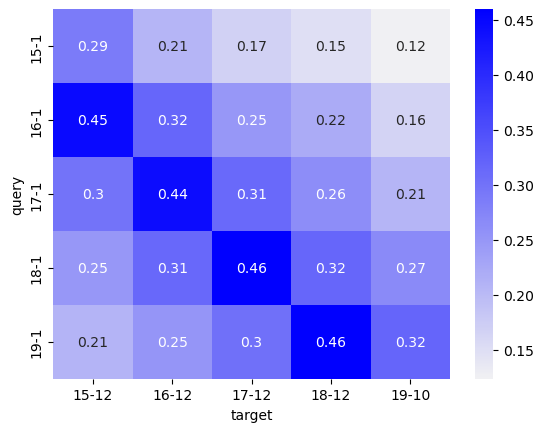
\includegraphics[width=\linewidth]{stylometryExtensions/figures/heat/sbert.png}
    \caption{SBERT}
    \label{fig:tempral_vary:sbert}
    \end{subfigure}

    
    \begin{subfigure}{0.48\linewidth}
    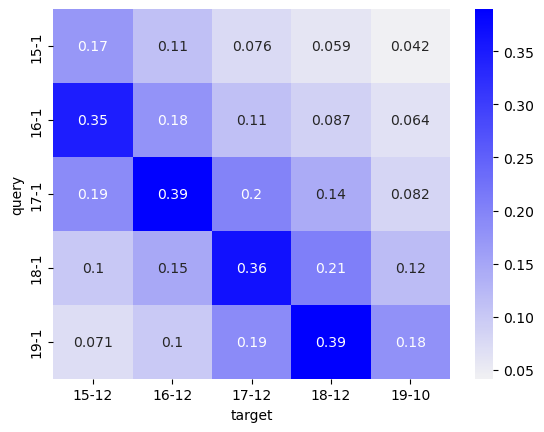
\includegraphics[width=\linewidth]{stylometryExtensions/figures/heat/stel.png}
    \caption{STEL}
    \label{fig:tempral_vary:stel}
    \end{subfigure}
    \begin{subfigure}{0.48\linewidth}
    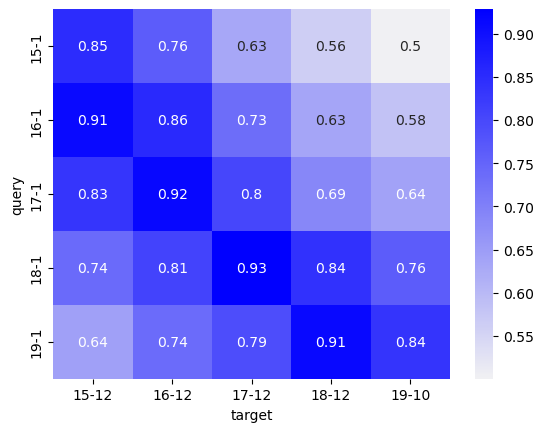
\includegraphics[width=\linewidth]{stylometryExtensions/figures/heat/luar.png}
    \caption{LUAR}
    \label{fig:tempral_vary:LUAR}
    \end{subfigure}

    \caption{Recall@8 results on \DSvarydelta{}}
    \label{fig:temporal_vary}
\end{figure}

\begin{figure}
    \centering
    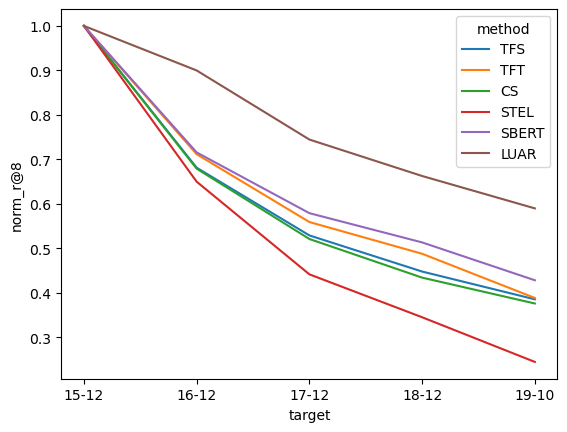
\includegraphics[width=0.6\textwidth]{stylometryExtensions/figures/luar_degradation.png}
    \caption{Target results for the earliest query split (15-1). We compare normalized recall@8 across all methods for \DSvarydelta{}.}
    \label{fig:temporal_vary:line}
\end{figure}
Next, using \DSvarydelta{} we consider temporal variation across a fixed set of users across time.
Figure~\ref{fig:temporal_vary} shows heatmaps for the recall@8 results for each model across different query/target time periods for a fixed set of authors.
We see that across all the methods, there is a temporal degradation in performance, which could potentially be caused by temporally evolving styles (STEL), topics of interest (Count/TFIDF) based results or semantics (SBERT).
However, from Figure~\ref{fig:temporal_vary:line}, we see that when normalized for diagnal, degradation in performance is the least for LUAR.
This indicates that the author representation features captured by LUAR are more stable across time compared to the other models.

\subsubsection{DemographicReddit}
\begin{figure}[h]
    \centering
    %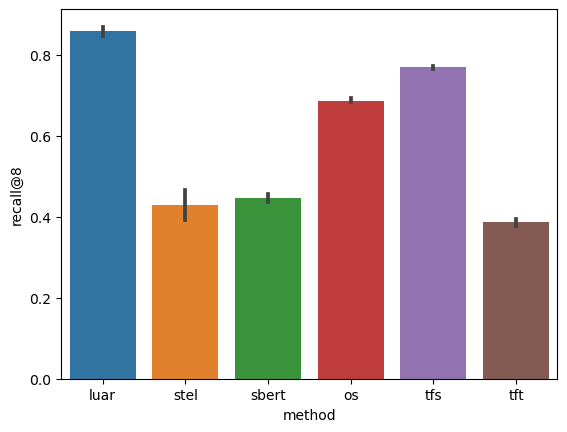
\includegraphics[width=0.48\linewidth]{stylometryExtensions/figures/demo/fixeddelta_demographics_age.png}
    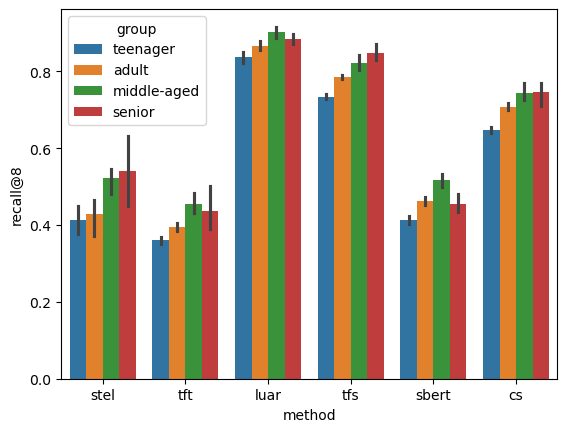
\includegraphics[width=0.6\textwidth]{stylometryExtensions/figures/demo/fixeddelta_demographics_age_groupwise.png}
    \caption{Overall results on \DSagefixed{} split by age group. }
    \label{fig:demographic_fixed:age}
\end{figure}
\begin{figure}[h]
    \centering
    %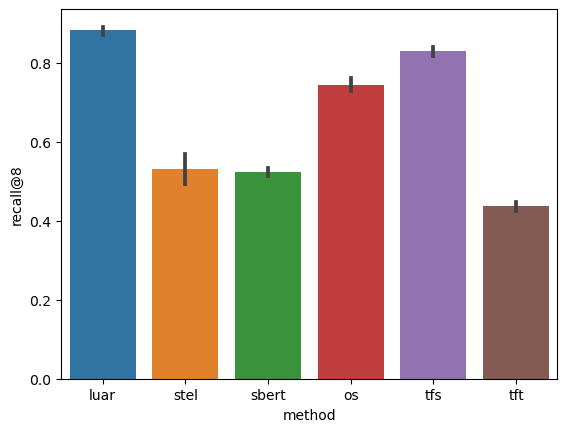
\includegraphics[width=0.48\linewidth]{stylometryExtensions/figures/demo/fixeddelta_demographics_gender.png}
    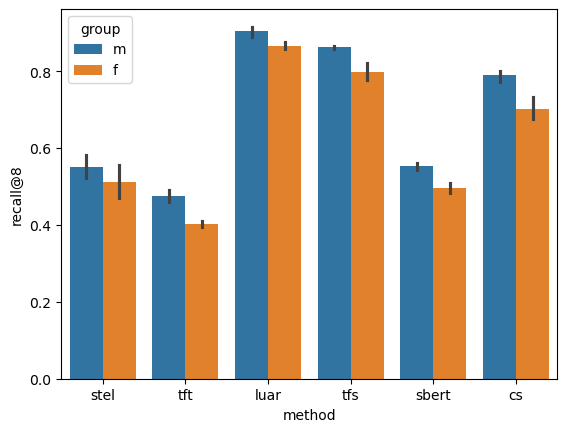
\includegraphics[width=0.6\textwidth]{stylometryExtensions/figures/demo/fixeddelta_demographics_gender_groupwise.png}
    \caption{Overall results on \DSgenderfixed{} split by each group (bottom).}
    \label{fig:demographic_fixed:gender}
\end{figure}
First, we consider the results for the demographic splits controlled for temporal variation.
Figure~\ref{fig:demographic_fixed:age} shows the recall@8 results for age groups across different models on \DSagefixed{}.
We note that all models consistently underperform on (self-identified) teenage users.
Further, from Figure~\ref{fig:demographic_fixed:gender}, we note that all models consistently underperform on (self-identified) female users.

\begin{figure}[h]
    \centering
    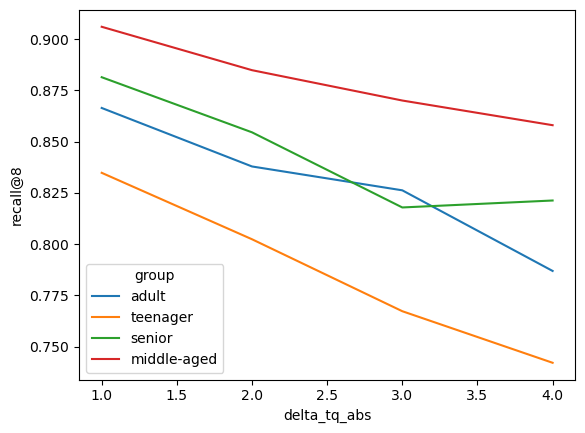
\includegraphics[width=0.6\textwidth]{stylometryExtensions/figures/demo/varydelta_demographic_groupwise_age.png}
    \caption{Overall results on \DSagevary{}. The x-axis denotes the absolute difference in the query and target start time, i.e., $|T_{\rm{start}} - Q_{\rm{start}}|$ .}
    \label{fig:demographic_vary:age}
\end{figure}

\begin{figure}[h]
    \centering
    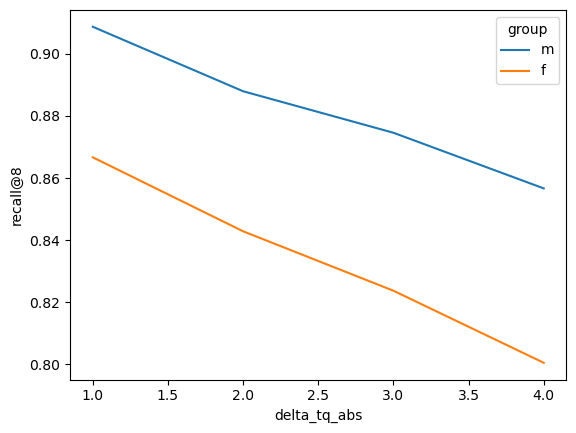
\includegraphics[height=0.6\textwidth]{stylometryExtensions/figures/demo/varydelta_demographic_groupwise_gender.png}
    \caption{Overall results on \DSgendervary{}. The x-axis denotes the absolute difference in the query and target start time, i.e., $|T_{\rm{start}} - Q_{\rm{start}}|$. }
    \label{fig:demographic_vary:gender}
\end{figure}

Next, we consider \DSagevary{} and \DSgendervary{}.
We focus on LUAR, as it is the best performing model across all the datasets.
The results from Figure~\ref{fig:demographic_vary:age} that across all $|T_{\rm{start}} - Q_{\rm{start}}|$, (self-identified) teenage authors are consistently the least identifiable.
Further, from Figure~\ref{fig:demographic_vary:gender}, We note that across all $|T_{\rm{start}} - Q_{\rm{start}}|$ and all models, authors self identifying as female are consistently the least identifiable.


\subsubsection{Analysis}
From the results with TemporalReddit, we can conclude that model estimation is unlikely to be a cause for the degradation in performance over time.
However, changing author interests and writing styles do contribute to the degradation in performance.
Drilling down into the specifics, we find that the degradation in performance is more significant for certain groups, notably younger authors and female authors.
Our results support our hypothesis that author representations encode systematic biases with respect to demographics. 
These biases get further exacerbated across time.
Care must be taken when deploying authorship attribution models in forensic applications, as the models may suffer from higher error rates and potential negative outcomes, such as false attributions, for certain the aforementioned groups.


\subsection{Limitations}
\citet{tigunova2020reddust} carefully extracted self-identified demographic traits while excluding posts made by users on subreddits involving gamin/roleplaying as authors tend to adopt different personas in such subreddits.
However, our analysis presupposes the correctness of their demographic extraction process.
The demographic traits are self-identified, and there is no way to verify the accuracy of these traits.
This limitation must be noted when interpreting the results from the TemporalReddit and DemographicReddit datasets.



%\subsubsection{Robustness}

%\pmComment{Uncomment below for probing results}
\begin{comment}
\subsubsection{Probing Classifier}
Two possible stories to explain the probing classifier results:
\begin{itemize}
    \item[1.] Performance is better for groups for which there is more training data. If most Reddit users are male, then the model will probably be better at identifying male authors, which may in turn improve the probing classifier's ability to distinguish gender.
    \item[2.] If style ranges widely across groups, there is nothing in particular for the representation to learn.
\end{itemize}

Comparing spread of ROC curves across groups: ...
\begin{figure*}[h]
\begin{subfigure}{.5\linewidth}
    \includegraphics[width=\linewidth]{figures/probe/roc_sepgender_luar.png}
    \caption{Probing classifier results for LUAR-Gender}
    \label{fig:probe_luargender_sep}
    \end{subfigure}
    \begin{subfigure}{.5\linewidth}
    \includegraphics[width=\linewidth]{figures/probe/roc_5folds_age_luar_v2.png}
    \caption{Probing classifier results for LUAR-Age}
    \label{fig:probe_luarage}
    \end{subfigure}
    
    \begin{subfigure}{.5\linewidth}
    \includegraphics[width=\linewidth]{figures/probe/roc_sepgender_sbert.png}
    \caption{Probing classifier results for SBERT-Gender}
    \label{fig:probe_sbertgender_sep}
    \end{subfigure}
    \begin{subfigure}{.5\linewidth}
    \includegraphics[width=\linewidth]{figures/probe/roc_5folds_age_sbert_v2.png}
    \caption{Probing classifier results for SBERT-Age}
    \label{fig:probe_sbertage}
    \end{subfigure}

    \begin{subfigure}{.5\linewidth}
    \includegraphics[width=\linewidth]{figures/probe/roc_sepgender_stel.png}
    \caption{Probing classifier results for STEL-Gender}
    \label{fig:probe_stelgender_sep}
    \end{subfigure}
    \begin{subfigure}{.5\linewidth}
    \includegraphics[width=\linewidth]{figures/probe/roc_5folds_age_stel_v2.png}
    \caption{Probing classifier results for STEL-Age}
    \label{fig:probe_stelage}
    \end{subfigure}
\end{figure*}

%%%%%%%%%%%%%%%%%%%%%%%%%%%%%%%%%%%%%%%%%%%%%%%%%
\begin{figure*}[h]\vspace{-1.6cm}
\begin{subfigure}{.33\linewidth}
    \includegraphics[width=\linewidth]{figures/probe/roc_ovo_age_luar_0.png}
    % \caption{\tiny OvO ROC for Age - LUAR}
    \label{fig:probe_ovoluarage}
    \end{subfigure}\vspace{-.35cm}
    \begin{subfigure}{.33\linewidth}
    \includegraphics[width=\linewidth]{figures/probe/roc_ovo_age_sbert_0.png}
    % \caption{\tiny OvO ROC for Age - SBERT}
    \label{fig:probe_ovosbertage}
    \end{subfigure}\vspace{-.35cm}
    \begin{subfigure}{.33\linewidth}
    \includegraphics[width=\linewidth]{figures/probe/roc_ovo_age_stel_0.png}
    % \caption{\tiny OvO ROC for Age - STEL}
    \label{fig:probe_ovostelage}
    \end{subfigure}\vspace{-.35cm}
\begin{subfigure}{.33\linewidth}
    \includegraphics[width=\linewidth]{figures/probe/roc_ovo_age_luar_1.png}
    \end{subfigure}\vspace{-.2cm}
    \begin{subfigure}{.33\linewidth}
    \includegraphics[width=\linewidth]{figures/probe/roc_ovo_age_sbert_1.png}
    \end{subfigure}\vspace{-.2cm}
    \begin{subfigure}{.33\linewidth}
    \includegraphics[width=\linewidth]{figures/probe/roc_ovo_age_stel_1.png}
    \end{subfigure}\vspace{-.2cm}
\begin{subfigure}{.33\linewidth}
    \includegraphics[width=\linewidth]{figures/probe/roc_ovo_age_luar_2.png}
    \end{subfigure}\vspace{-.2cm}
    \begin{subfigure}{.33\linewidth}
    \includegraphics[width=\linewidth]{figures/probe/roc_ovo_age_sbert_2.png}
    \end{subfigure}\vspace{-.2cm}
    \begin{subfigure}{.33\linewidth}
    \includegraphics[width=\linewidth]{figures/probe/roc_ovo_age_stel_2.png}
    \end{subfigure}\vspace{-.2cm}
\begin{subfigure}{.33\linewidth}
    \includegraphics[width=\linewidth]{figures/probe/roc_ovo_age_luar_3.png}
    \end{subfigure}\vspace{-.2cm}
    \begin{subfigure}{.33\linewidth}
    \includegraphics[width=\linewidth]{figures/probe/roc_ovo_age_sbert_3.png}
    \end{subfigure}\vspace{-.2cm}
    \begin{subfigure}{.33\linewidth}
    \includegraphics[width=\linewidth]{figures/probe/roc_ovo_age_stel_3.png}
    \end{subfigure}\vspace{-.2cm}
\begin{subfigure}{.33\linewidth}
    \includegraphics[width=\linewidth]{figures/probe/roc_ovo_age_luar_4.png}
    \end{subfigure}\vspace{-.2cm}
    \begin{subfigure}{.33\linewidth}
    \includegraphics[width=\linewidth]{figures/probe/roc_ovo_age_sbert_4.png}
    \end{subfigure}\vspace{-.2cm}
    \begin{subfigure}{.33\linewidth}
    \includegraphics[width=\linewidth]{figures/probe/roc_ovo_age_stel_4.png}
    \end{subfigure}\vspace{-.2cm}
\begin{subfigure}{.33\linewidth}
    \includegraphics[width=\linewidth]{figures/probe/roc_ovo_age_luar_5.png}
    \end{subfigure}\vspace{-.3cm}
    \begin{subfigure}{.33\linewidth}
    \includegraphics[width=\linewidth]{figures/probe/roc_ovo_age_sbert_5.png}
    \end{subfigure}\vspace{-.3cm}
    \begin{subfigure}{.33\linewidth}
    \includegraphics[width=\linewidth]{figures/probe/roc_ovo_age_stel_5.png}
    \end{subfigure}\vspace{-.3cm}
\end{figure*}

%%%%%%%%%%%%%%%%%%%%%%%%%%%%%%%%%%%%%%%%%%%%%%%%%
\begin{figure*}[h]
\begin{subfigure}{.33\linewidth}
    \includegraphics[width=\linewidth]{figures/probe/roc_5folds_gender_luar.png}
    \caption{\tiny Probing classifier results for LUAR-Gender1}
    \label{fig:probe_luargender}
    \end{subfigure}
    \begin{subfigure}{.33\linewidth}
    \includegraphics[width=\linewidth]{figures/probe/roc_5folds_gender_sbert.png}
    \caption{\tiny Probing classifier results for SBERT-Gender1}
    \label{fig:probe_sbertgender}
    \end{subfigure}
    \begin{subfigure}{.33\linewidth}
    \includegraphics[width=\linewidth]{figures/probe/roc_5folds_gender_stel.png}
    \caption{\tiny Probing classifier results for STEL-Gender1}
    \label{fig:probe_stelgender}
    \end{subfigure}
\end{figure*}
    
% \begin{figure*}
%     \centering
%     \includegraphics[width=\linewidth]{figures/probe/roc_5folds_gender_luar.png}
%     \includegraphics[width=\linewidth]{figures/probe/roc_5folds_gender_sbert.png}
%     \caption{}
%     \label{fig:probe_gender}
% \end{figure*}

% \begin{figure*}
%     \centering
%     \includegraphics[width=\linewidth]{figures/probe/roc_5folds_age_luar.png}
%     \includegraphics[width=\linewidth]{figures/probe/roc_5folds_age_sbert.png}
%     \caption{}
%     \label{fig:probe_age}
% \end{figure*}
%%%%%%%%%%%%%%%%%%%%%%%%%%%%%%%%%%%%%%%%%%%%%%%%%
\end{comment}